\documentclass[twocolumn]{article}
\usepackage[utf8]{inputenc}

\usepackage[backend=bibtex,style=ieee]{biblatex}
\bibliography{biblio_dvs_emu_paper}

\usepackage{graphicx}
\graphicspath{{./pictures/}}


%\usepackage{multicol}

%opening
\title{A Real-time Dynamic Vision Sensor Emulator using Off-the-shelf Hardware}
\author{Garibaldi Pineda García}



\begin{document}

\maketitle
%\begin{multicols}{2}
%[
  \begin{abstract}
  Vision is one of our most important senses, a vast amount of information is perceived through our eyes. Neuroscientists have performed several studies using vision as input to their experiments. However, computational neuroscience has typically used Poisson-encoded images as spike-based visual sources. Recently neuromorphic Dynamic Vision Sensors have surfaced, while they have excellent capabilities, they remain scarce and difficult to use.
  
  We propose a software-based visual input system, inspired by the behaviour of a DVS, but using a digital camera as a sensor. By using readily-available components, we believe, most scientist would have access to a spiking visual input source. While the primary goal was to use the system as a real-time input, it is also able to transcode well established images and video databases into spike train representations. Our main contributions are adding locally inhibitory behaviour, adaptive thresholds and proposing time-based encoding of the output spikes.
  
  \end{abstract}
%]

  \section{Introduction}
  
  In recent years the performance of computer processors has been advancing in smaller increments than it used to a few years ago. This is mainly because manufacturing technologies are reaching their limits. One way to improve performance is to use many processors in parallel, which has been successfully applied to parallel-friendly applications like computer graphics. Task like pattern recognition are still a hard task for computers even with these technological advances.
  
  Our brains are particularly good at learning and recognizing visual patterns (e.g. letters, dogs, houses, etc.). In order to achieve better performance for similar tasks on computers, scientists have looked into biology for inspiration. This has lead to the rise of brain-like (neuromorphic) hardware, which looks to mimic functional aspects of the nervous system. We can divide neuromorphic hardware into sensors (providing input) and computing devices (make use of information from sensors). Visual input has been traditionally obtained from images that are rate-encoded using Poisson processes, while this might be a biologically-plausible encoding in the first phase of a ``visual pipeline'' it is unlikely that eyes transmit as much information into later stages. Furthermore, if we think of it in terms of digital networks, having each pixel represented by a Poisson process incurs in high bandwidth requirements. 
  
  In \citeyear{Mead1989}, \citeauthor{Mead1989} proposed a silicon retina consisting of individual photoreceptors and a resistor mesh that allowed nearby receptors to influence on the output of a pixel~\cite{Mead1989}. 
  Later, researchers developed frame-free Dynamic Vision Sensors (DVSs)~\cite{delbruck_dvs,bernabe_dvs}. They feature independent pixels that emit a signal when its intensity value changes above a certain threshold. These sensors have $\mu$-second response time and excellent dynamic range properties, although they are still not as commercially available as regular cameras.
  
  In this work, we propose to emulate the behaviour of a DVS using a conventional digital camera as a sensor. Basing the emulator on widely available hardware, would allow most computational neuroscientists to include video as a spike-based input.
  
  
  \citeauthor{dvs_emu} developed a DVS emulator in order to test behaviours for new sensor models~\cite{dvs_emu}. In their work, they transform the image provided a commercial camera into a spike stream at 125 frames per second (fps). In simple terms, the emulation is done by differencing video input with a reference frame; if this difference is larger than a threshold it produces an output and updates the reference. The number of spikes produced per pixel are proportional to how many times the difference would pass the threshold. This emulator has been merged into the jAER project, a Java-based Address-Event Representation software framework that specializes on processing DVS output in real time.
  
  
  \section{Work}
  
  Pixels in DVSs are independent and transform light input into a logarithmic representation. Most commercial cameras produce gamma-encoded images~\cite{Poynton_digital_video} to better utilize bits and, in older days, to be compliant with cathode ray tube (CRT) monitors. Figure~\ref{fig:gamma_coding} shows the response for the encoding process (crosses), CRT monitors (hexagons) and decoding process (dots). Since the encoding response is similar to the logarithmic used in the DVS, we skip this step of the emulation.
  
  \begin{figure}[htb]
    \includegraphics[width=0.5\textwidth]{gamma_coding}
    \label{fig:gamma_coding}
    \caption{Gamma encoding and decoding functions, $\gamma = 2.2$}
  \end{figure}
  
  Asynchronous pixel behaviour is approximated via differencing the current image obtained by the camera and a reference frame; whenever a pixel's difference is larger than a certain threshold, we mark that position as ``spiked''. Depending on the selected type of output we simulate a receiver and update the reference accordingly. This is the basic DVS emulation and it's illustrated in Figure~\ref{fig:dvs_emu}.
  
  \begin{figure}[htb]
    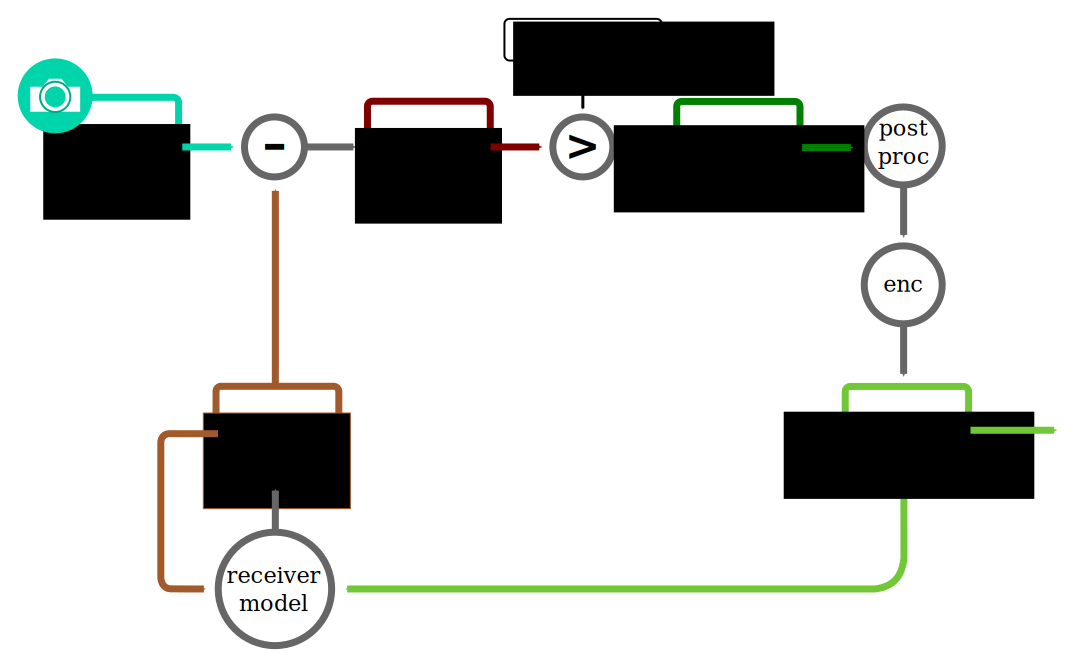
\includegraphics[width=0.5\textwidth]{dvs_emu}
    \label{fig:dvs_emu}
    \caption{DVS emulation diagram. Circles indicate operations and rectangles states of data}
  \end{figure}
  
  \subsection{Output modes}
  \subsubsection{Rate-based}
  As in previous emulators\cite{dvs_emu}, the standard output format is rate-based. In this mode each spike can be interpreted as an increment or decrement in intensity. To calculate the number of spikes that represent we use the following expression
  \begin{equation}
    \label{eq:num_spikes_rate}
    N_{s} = \left\lfloor \frac{\Delta I}{H} \right\rfloor
  \end{equation}
  where $N_{s}$ is the number of spikes needed to represent the change in intensity $\Delta I$ in terms of the threshold $H$. At this stage we model the perfect receiver, so the quantity that will update the reference is
  \begin{equation}
    \label{eq:ref_update}
    \Delta R = N_{s}\times H
  \end{equation}
  %Notice that since we are using the signed difference in Eq. \ref{eq:num_spikes_rate}, the update $\Delta R$ is also signed.
  
  \subsubsection{Time-based}
  In its worst case rate-based encoding can send a spike per millisecond per pixel, which can potentially saturate communication channels. One way to prevent this is to encode the value that each spike represents by the time each spike is sent. First we propose to encode the number of times the threshold would have been exceeded~(Eq.~\ref{eq:num_spikes_rate}), Figure~\ref{fig:linear_time} shows the value to time relation, in our proposal earlier spikes represent larger changes in intensity. The main advantage of this encoding is that a single spike could represent multiple rate-based spikes, though the encoded values are limited by the time resolution and the frame rate of the camera.
  
  \begin{figure}[htb]
    \includegraphics[width=0.5\textwidth]{spike_stream_time}
    \label{fig:linear_time}
    \caption{Linear time-based encoding of spikes number}
  \end{figure} 
  
  In order to decode spikes from the receiver side we must keep track of the last time a spike was collected (Eq.). 
  % record the last time a spike was received and calculate the difference with the current time. Finally we obtain the remainder of the division of the difference and the inter-frame time.
  \begin{equation}
    \label{eq:decode_time}
    \Delta I_o = \mathrm{mod}\left(t_{now} - t_{last}, T\right)\times H
  \end{equation}
  where $\Delta I_o$ is the change in intensity derived from the spike stream, $t_{now}$ is the time when the current spike arrived, $t_{last}$ is the time last spike was received, $T$ is the inverse of the camera's frames per second, and $\mathrm{mod}$ calculates the arguments' division remainder.
  
  To overcome the limitation of encoded values we propose binary encoding of either the absolute difference in intensity or the number of thresholds exceeded. 
  We propose different time encodings (raw value/binary, threshold multiples/binary, threshold multiples/linear)\\
  
  \subsection{Additional behaviours}
  \subsubsection{Local inhibition} reduces bandwidth, persistence of spatial stimuli over frames. 
  \subsubsection{Adaptive threshold} slow-charging pixels by reducing the threshold.\\
  Less parameters to configure.
  \subsubsection{History decay}
  Open source, and available in github.com\\
  
  \section{Results}
  
  Real-time DVS emulation on consumer hardware (Intel i5, 8GB ram)
  sPyNNaker wrapper for videos and images.
  
  \section{Conclusion}
  
  GPU computing version would allow for higher resolutions.
  
  Working on ganglion cell/Difference of Gaussian encoding.
  
  \printbibliography
%\end{multicols}
\end{document}
